\newpage
\section{Application to Fusion Simulation Data}
\label{sec:xgc}
We report on our application to fusion simulation data from the XGC
code \cite{??}. The resulting data has 480 time steps, each with 32
equispaced polloidal slices. We perform 4 PCA decompositions of the
{\it density potential} (dpot) variable indexed by time steps 100,
200, 300, and 400, by taking the index time step and 15 more steps
following it to get a total of $32\times 16$ slices, each with 232,011
gridpoints. This results in a $256\times 232,011$ matrix, which is
very skinny and takes roughly 1 GB memory.

The decision to construct the PCA input matrix as described is
motivated by the need to view its rows as sample points from a
stationary distribution. It is reasonable to assume that the slices in
a single time step are from the same high dimensional (specifically,
232,011 dimensional) distribution that can be characterized by its top
principal components.

\subsection{Computation with Fast Skinny PCA Algorithm}
Our algorithm is implemented in R with pbdR infrastructure
\cite{Schmidt2017}, which for the specific skinny matrix computations
is a workflow driving MPI, LAPACK, BLAS, and ADIOS library
support. Our runs are done on Oak Redge Leadership Computing
Facility's (OLCF) Rhea, which is a 512 node commodity cluster with
dual Intel® Xeon® E5-2650 @ 2.0 GHz giving 16 cores per node.

Running on 8 nodes (128 cores), it takes
approximately 6 to 8 seconds to read the data from a lustre file
system, and under 2 seconds to perform the decomposition. Production
of the 512 resulting plots of right singular vectors and scree plots, like
those shown in Figures~\ref{fig:100} to \ref{fig:400}, takes roughly
100 seconds.

We expect that the resulting speeds are more than sufficient to keep
up with a running XGC simulation, which takes roughly four seconds per
time step \cite{XGCpertimestep}, giving 64 seconds for our 16 step
ensemble. We envision the decomposition code running as a service
connected to an ADIOS in memory staging file system. In this service
scenario, reading the data should be faster than what we experience
here from a lustre file system. Also, instead of producing plots, the
decomposed data reduced to some smaller number of components ($\ll$
512) would be output to the file system in a time that would be less
than the 6 to 8 seconds taken here to read the data. Next, we comment
on the results in Figures~\ref{fig:100} to \ref{fig:400}.
\begin{figure}[tbp]
  \begin{center}
    \slc{0.245}{Figs/p100/pc00001.00100.png}
    \slc{0.245}{Figs/p100/pc00002.00100.png}
    \slc{0.245}{Figs/p100/pc00003.00100.png}
    \slc{0.245}{Figs/p100/pc00004.00100.png}\\
    \slc{0.245}{Figs/p100/pc00005.00100.png}
    \slc{0.245}{Figs/p100/pc00006.00100.png}
    \slc{0.245}{Figs/p100/pc00007.00100.png}
    \slc{0.245}{Figs/p100/pc00008.00100.png}\\
    \slc{0.245}{Figs/p100/pc00009.00100.png}
    \slc{0.245}{Figs/p100/pc00010.00100.png}
    \slc{0.245}{Figs/p100/pc00011.00100.png}
    \slc{0.245}{Figs/p100/pc00012.00100.png}\\
    \slc{0.245}{Figs/p100/pc00013.00100.png}
    \slc{0.245}{Figs/p100/pc00014.00100.png}
    \slc{0.245}{Figs/p100/pc00015.00100.png}
    \slc{0.245}{Figs/p100/pc00016.00100.png}\\
    \slc{0.245}{Figs/p100/pc00017.00100.png}
    \slc{0.245}{Figs/p100/pc00018.00100.png}
    \slc{0.245}{Figs/p100/pc00019.00100.png}
    \slc{0.245}{Figs/p100/pc00020.00100.png}\\
    \slc{0.245}{Figs/p100/pc00021.00100.png}
    \slc{0.245}{Figs/p100/pc00022.00100.png}
    \slc{0.245}{Figs/p100/pc00023.00100.png}
    \slc{0.245}{Figs/p100/pc00024.00100.png}\\
    \scr{0.35}{Figs/p100/scree.pdf}
    \scr{0.35}{Figs/p100/scree100log.pdf}
  \end{center}
  \caption{Time steps 100 to 115}
  \label{fig:100}
\end{figure}

\begin{figure}[tbp]
  \begin{center}
    \slc{0.245}{Figs/p200/pc00001.00200.png}
    \slc{0.245}{Figs/p200/pc00002.00200.png}
    \slc{0.245}{Figs/p200/pc00003.00200.png}
    \slc{0.245}{Figs/p200/pc00004.00200.png}\\
    \slc{0.245}{Figs/p200/pc00005.00200.png}
    \slc{0.245}{Figs/p200/pc00006.00200.png}
    \slc{0.245}{Figs/p200/pc00007.00200.png}
    \slc{0.245}{Figs/p200/pc00008.00200.png}\\
    \slc{0.245}{Figs/p200/pc00009.00200.png}
    \slc{0.245}{Figs/p200/pc00010.00200.png}
    \slc{0.245}{Figs/p200/pc00011.00200.png}
    \slc{0.245}{Figs/p200/pc00012.00200.png}\\
    \slc{0.245}{Figs/p200/pc00013.00200.png}
    \slc{0.245}{Figs/p200/pc00014.00200.png}
    \slc{0.245}{Figs/p200/pc00015.00200.png}
    \slc{0.245}{Figs/p200/pc00016.00200.png}\\
    \slc{0.245}{Figs/p200/pc00017.00200.png}
    \slc{0.245}{Figs/p200/pc00018.00200.png}
    \slc{0.245}{Figs/p200/pc00019.00200.png}
    \slc{0.245}{Figs/p200/pc00020.00200.png}\\
    \slc{0.245}{Figs/p200/pc00021.00200.png}
    \slc{0.245}{Figs/p200/pc00022.00200.png}
    \slc{0.245}{Figs/p200/pc00023.00200.png}
    \slc{0.245}{Figs/p200/pc00024.00200.png}\\
    \scr{0.35}{Figs/p200/scree.pdf}
    \scr{0.35}{Figs/p200/scree100log.pdf}
  \end{center}
  \caption{Time steps 200 to 215}
  \label{fig:200}
\end{figure}

\begin{figure}[tbp]
  \begin{center}
    \slc{0.245}{Figs/p300/pc00001.00300.png}
    \slc{0.245}{Figs/p300/pc00002.00300.png}
    \slc{0.245}{Figs/p300/pc00003.00300.png}
    \slc{0.245}{Figs/p300/pc00004.00300.png}\\
    \slc{0.245}{Figs/p300/pc00005.00300.png}
    \slc{0.245}{Figs/p300/pc00006.00300.png}
    \slc{0.245}{Figs/p300/pc00007.00300.png}
    \slc{0.245}{Figs/p300/pc00008.00300.png}\\
    \slc{0.245}{Figs/p300/pc00009.00300.png}
    \slc{0.245}{Figs/p300/pc00010.00300.png}
    \slc{0.245}{Figs/p300/pc00011.00300.png}
    \slc{0.245}{Figs/p300/pc00012.00300.png}\\
    \slc{0.245}{Figs/p300/pc00013.00300.png}
    \slc{0.245}{Figs/p300/pc00014.00300.png}
    \slc{0.245}{Figs/p300/pc00015.00300.png}
    \slc{0.245}{Figs/p300/pc00016.00300.png}\\
    \slc{0.245}{Figs/p300/pc00017.00300.png}
    \slc{0.245}{Figs/p300/pc00018.00300.png}
    \slc{0.245}{Figs/p300/pc00019.00300.png}
    \slc{0.245}{Figs/p300/pc00020.00300.png}\\
    \slc{0.245}{Figs/p300/pc00021.00300.png}
    \slc{0.245}{Figs/p300/pc00022.00300.png}
    \slc{0.245}{Figs/p300/pc00023.00300.png}
    \slc{0.245}{Figs/p300/pc00024.00300.png}\\
    \scr{0.35}{Figs/p300/scree.pdf}
    \scr{0.35}{Figs/p300/scree100log.pdf}
  \caption{Time steps 300 to 315}
  \end{center}
  \label{fig:300}
\end{figure}

\begin{figure}[tbp]
  \begin{center}
    \slc{0.245}{Figs/p400/pc00001.00400.png}
    \slc{0.245}{Figs/p400/pc00002.00400.png}
    \slc{0.245}{Figs/p400/pc00003.00400.png}
    \slc{0.245}{Figs/p400/pc00004.00400.png}\\
    \slc{0.245}{Figs/p400/pc00005.00400.png}
    \slc{0.245}{Figs/p400/pc00006.00400.png}
    \slc{0.245}{Figs/p400/pc00007.00400.png}
    \slc{0.245}{Figs/p400/pc00008.00400.png}\\
    \slc{0.245}{Figs/p400/pc00009.00400.png}
    \slc{0.245}{Figs/p400/pc00010.00400.png}
    \slc{0.245}{Figs/p400/pc00011.00400.png}
    \slc{0.245}{Figs/p400/pc00012.00400.png}\\
    \slc{0.245}{Figs/p400/pc00013.00400.png}
    \slc{0.245}{Figs/p400/pc00014.00400.png}
    \slc{0.245}{Figs/p400/pc00015.00400.png}
    \slc{0.245}{Figs/p400/pc00016.00400.png}\\
    \slc{0.245}{Figs/p400/pc00017.00400.png}
    \slc{0.245}{Figs/p400/pc00018.00400.png}
    \slc{0.245}{Figs/p400/pc00019.00400.png}
    \slc{0.245}{Figs/p400/pc00020.00400.png}\\
    \slc{0.245}{Figs/p400/pc00021.00400.png}
    \slc{0.245}{Figs/p400/pc00022.00400.png}
    \slc{0.245}{Figs/p400/pc00023.00400.png}
    \slc{0.245}{Figs/p400/pc00024.00400.png}\\
    \scr{0.35}{Figs/p400/scree.pdf}
    \scr{0.35}{Figs/p400/scree100log.pdf}
  \caption{Time steps 400 to 415}
  \label{fig:400}
  \end{center}
\end{figure}

The bottom two scree graphs in each figure show the eigenvalues (squares of
the singular values) in decreasing order. The left graph shows all 512
eigenvalues on a linear scale and the right graph shows the top 50
eigenvalues on a log10 scale.

The right singular vectors correspond to and are plotted on the
polloidal slice gridpoints, producing the circular images in the
figures. Each image in reading order (left to right and then top to
bottom) corresponds to the eigenvalues in decreasing order. The units
of the displayed vectors are the same as for density potential (dpot)
and the legend to the
right of each shows the dpot values that correspond to the colors.

We have the following observations about the figures:
\begin{itemize}
\item The eigenvalues are usually paired and possibly in larger groups
  with larger steps between groups. It may be possible to interpret
  the groups as various wave energy representations.
\item Each of the time steps has a somewhat different decomposition
  but there common modes that occurr at different energy levels.
\item The eigenvalues decrease rapidly so that singular vectors beyond
  about 100 contribute very little to the variability and may
  represent noise. As a result, arguably only the singular vectors and
  their weights need to be output to reconstruct the simulation. This
  is a roughly $5\times$ reduction.
\end{itemize}

\subsection{Relationship to Tensor Decomposition}
Because our row dimension includes both time and space (toroidal angle
by time: $32\times 16$), there is a relationship between this
``stacked'' matrix PCA decomposition and the three dimensional tensor
($32\times 16\times 232,011$) decomposition. Namely, the stacked left
singular vectors ($32\times 16 = 512$) along with the spatial patterns
of the right singular vectors are the first iteration of the tensor
decomposition, sometimes referred to as the higher order singular
value decomposition (HOSVD) \cite[p.1264]{DeLathauwer2000}. That is,
the right singular vectors from our SVD, displayed as images, are the
rightmost singular 
vectors of the HOSVD. Here we describe some initial tensor
decomposition results for a similar but smaller data set.

The smaller data set, generated from one of small size XGC runs, is prepared as a 3-dimensional tensor, size of  $32\times20\times20,694$. We apply tensor decomposition in the context of data reduction, in which we decompose 3-d matrix with SVD-based tensor decomposition and reconstruct by using only a small subset of components. We compare the data reduction qualities, such as compression ratios and relative errors, depending on the number of components. Figure~\ref{fig:tensor-xgc} shows a series of XGC data reconstructed after tensor decomposition, by using different number of components, ranging from 1 and up to 10.

\begin{figure}[!h]
  \centering
  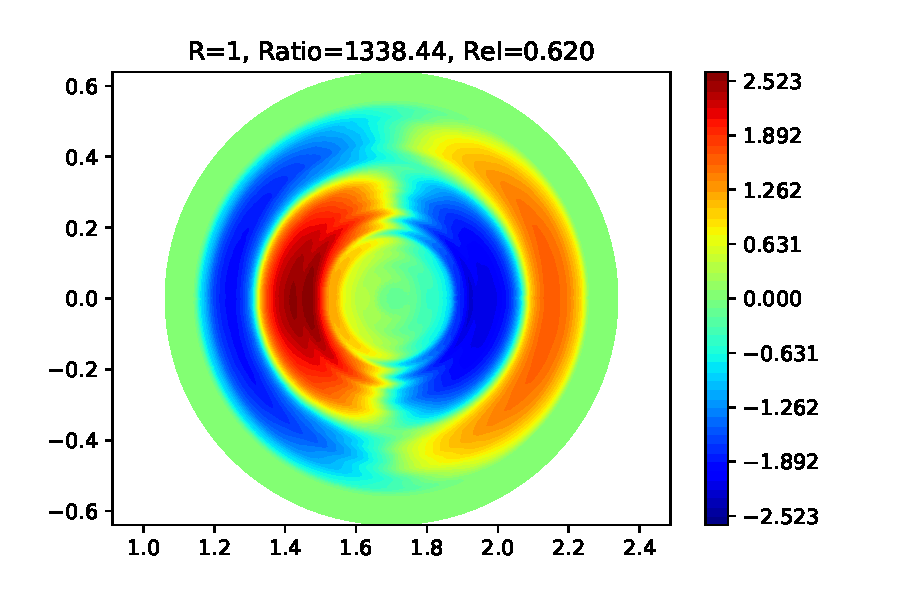
\includegraphics[width=0.32\linewidth]{Figs/tensor-1.pdf}
  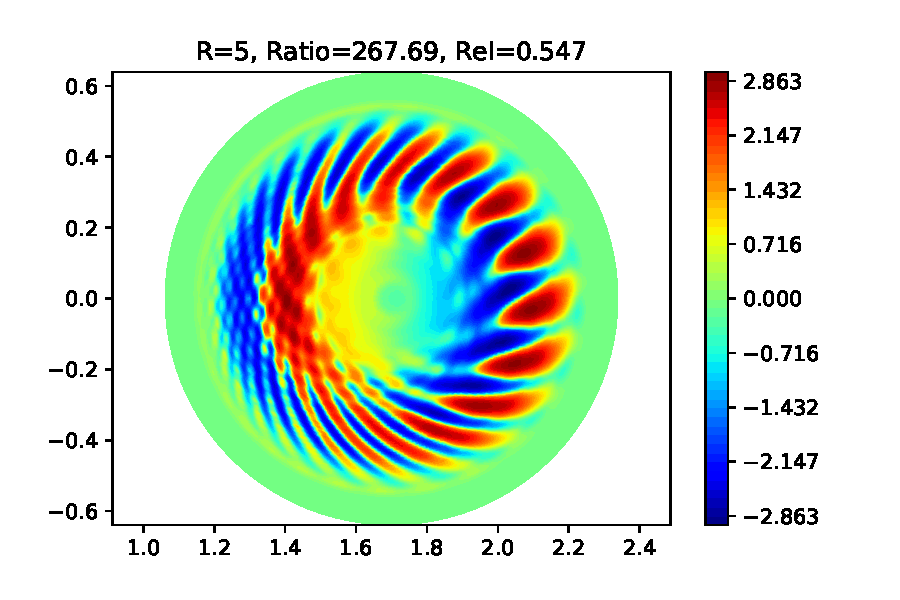
\includegraphics[width=0.32\linewidth]{Figs/tensor-5.pdf}
  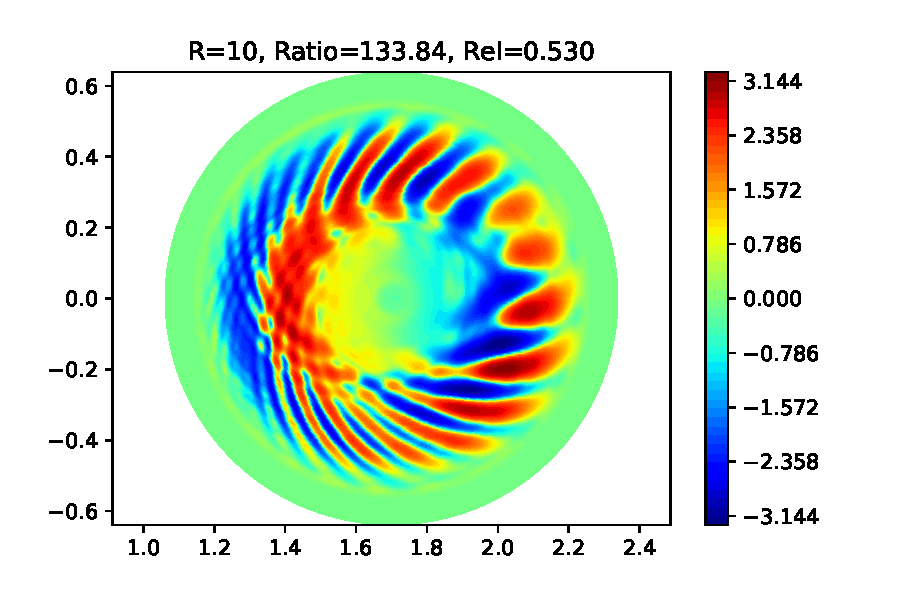
\includegraphics[width=0.32\linewidth]{Figs/tensor-10.pdf}
  \caption{Tensor decomposition of XGC field data. Images are reconstructed after applying SVD-based tensor decomposition. Different number of components are used, ranging from 1 (left) up to 10 (right). Compression ratios and relative errors are shown in the top.}
  \label{fig:tensor-xgc}
\end{figure}

\newpage
\subsection{Data Transformations Useful for PCA}
\subsection{Box-Cox and Symmetric Power Transformations}

\begin{figure}[!h]
  \centering
  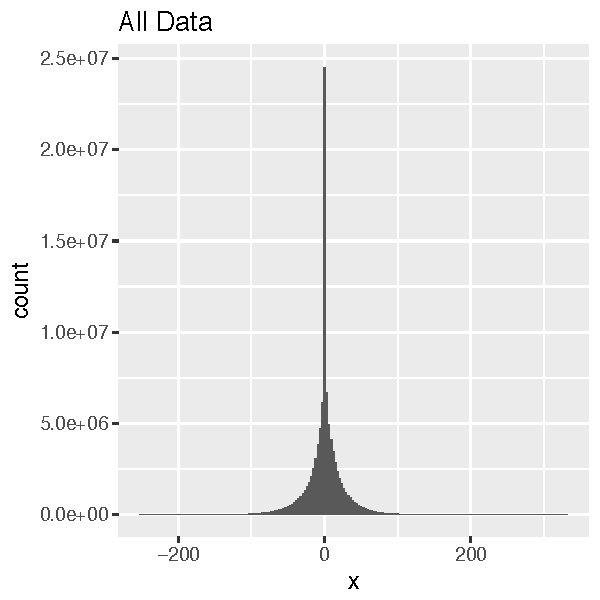
\includegraphics[width=0.16\linewidth]{Figs/raw}
  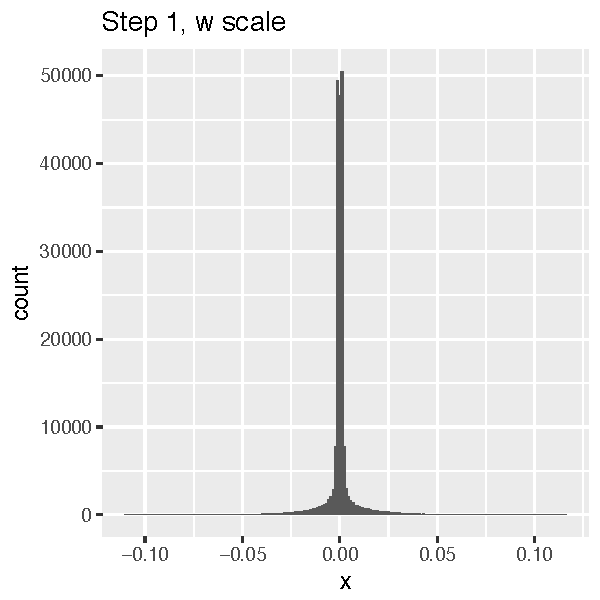
\includegraphics[width=0.16\linewidth]{Figs/raw_1}
  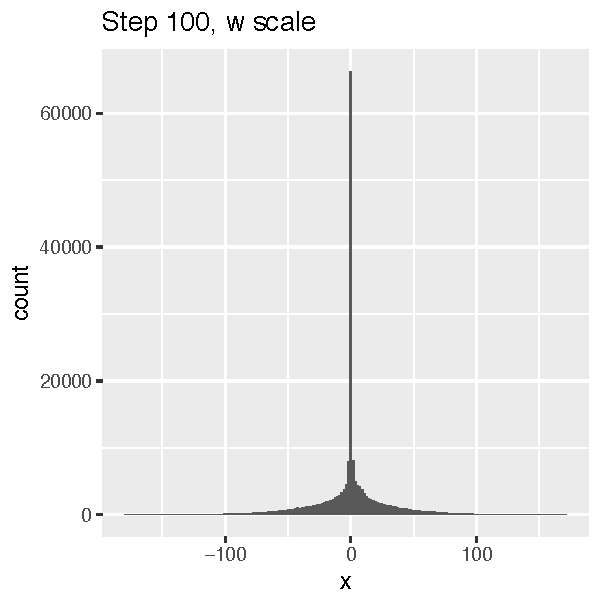
\includegraphics[width=0.16\linewidth]{Figs/raw_100}
  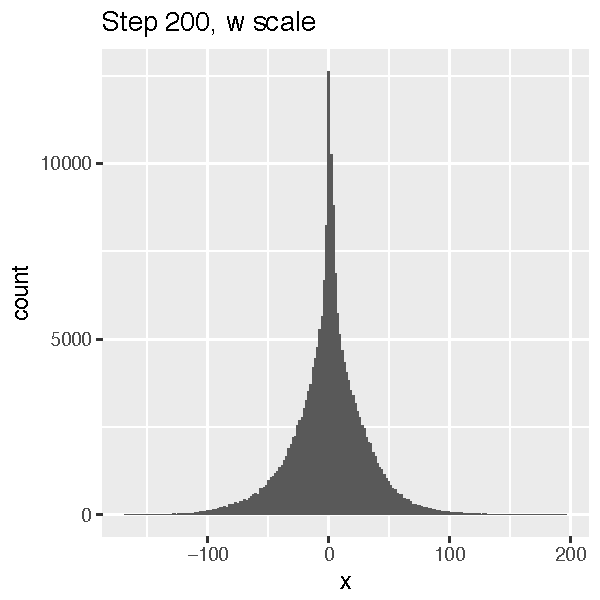
\includegraphics[width=0.16\linewidth]{Figs/raw_200}
  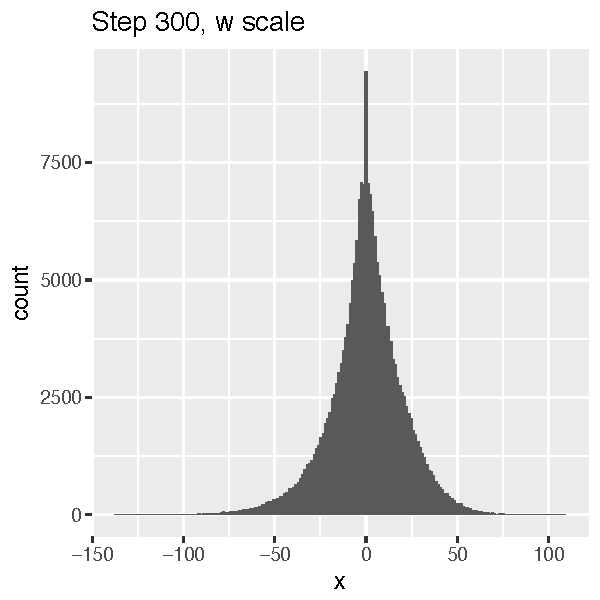
\includegraphics[width=0.16\linewidth]{Figs/raw_300}
  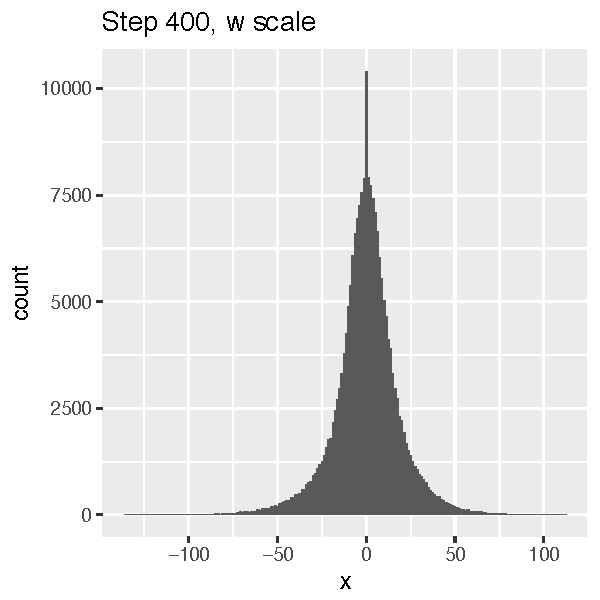
\includegraphics[width=0.16\linewidth]{Figs/raw_400}
  \caption{Histogram of all data followed by a few individual time steps.}
  \label{fig:hist_raw}
\end{figure}

\begin{equation}
  w = sign(x) |x|^{1/5}
\end{equation}

\begin{figure}[!h]
  \centering
  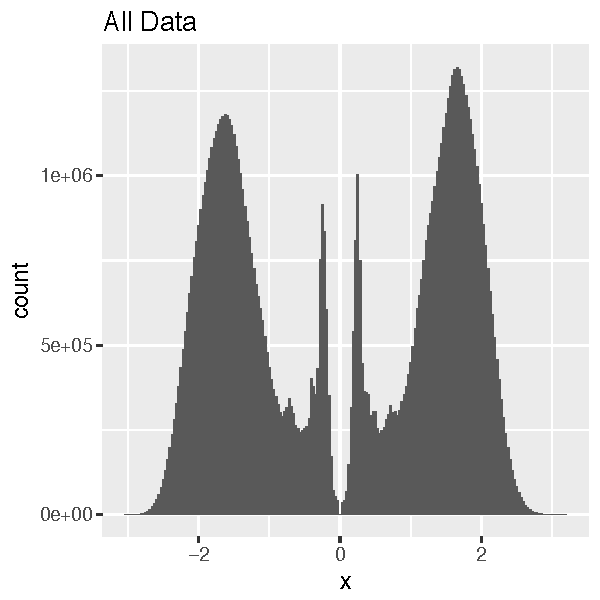
\includegraphics[width=0.16\linewidth]{Figs/tr}
  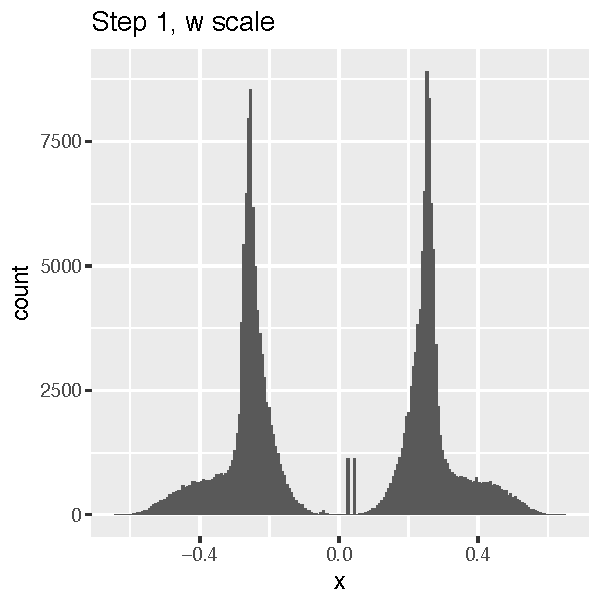
\includegraphics[width=0.16\linewidth]{Figs/tr_1}
  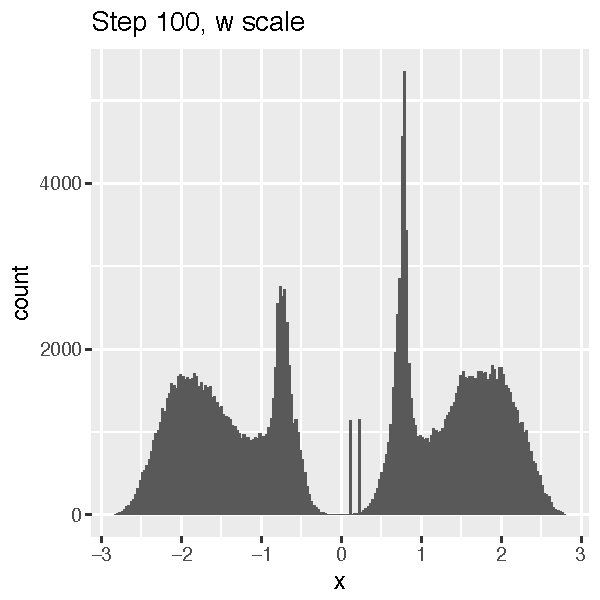
\includegraphics[width=0.16\linewidth]{Figs/tr_100}
  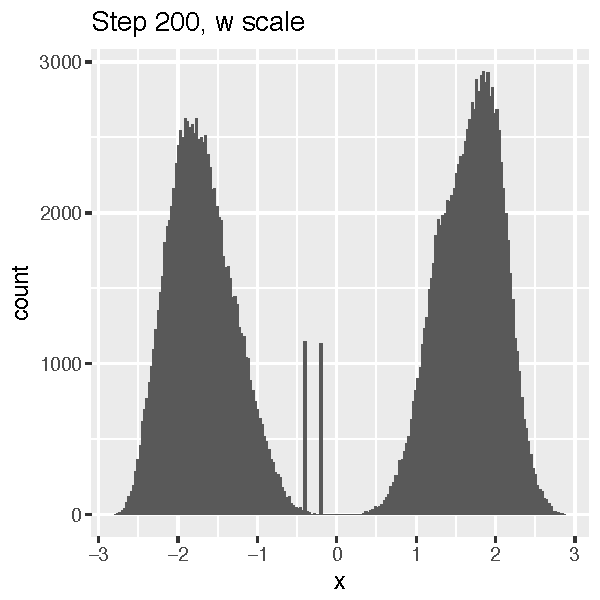
\includegraphics[width=0.16\linewidth]{Figs/tr_200}
  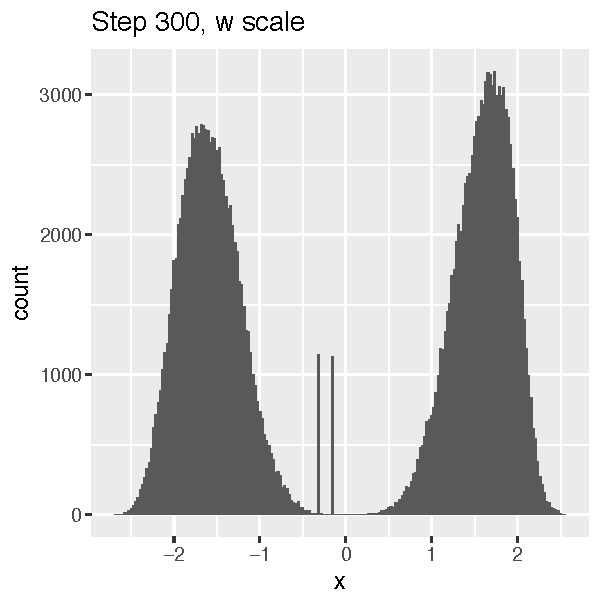
\includegraphics[width=0.16\linewidth]{Figs/tr_300}
  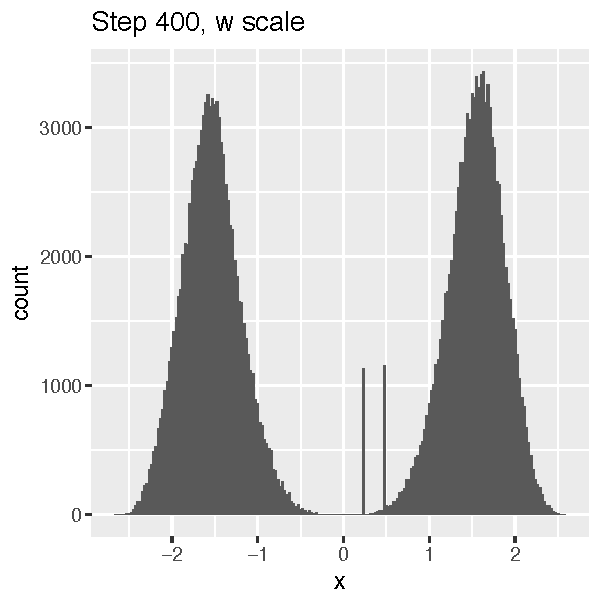
\includegraphics[width=0.16\linewidth]{Figs/tr_400}
  \caption{Same histograms as in Fig.~\ref{fig:hist_raw} after
    removing exact zeroes and transformation to $w$.}
  \label{fig:hist_tr}
\end{figure}

\begin{figure}[!h]
  \centering
  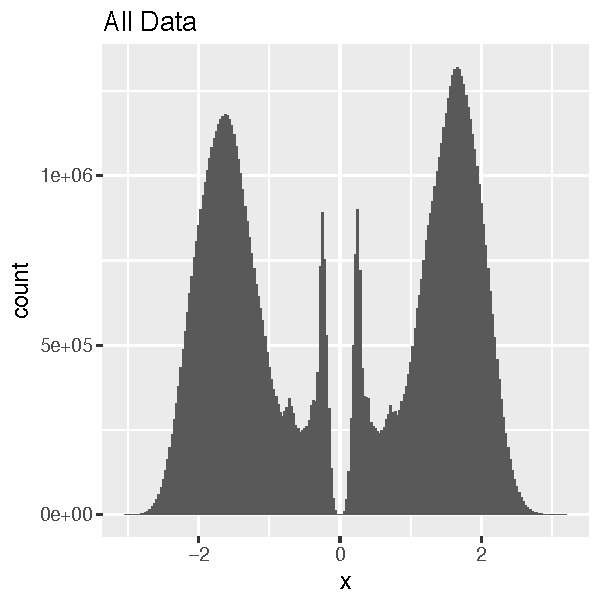
\includegraphics[width=0.16\linewidth]{Figs/trc}
  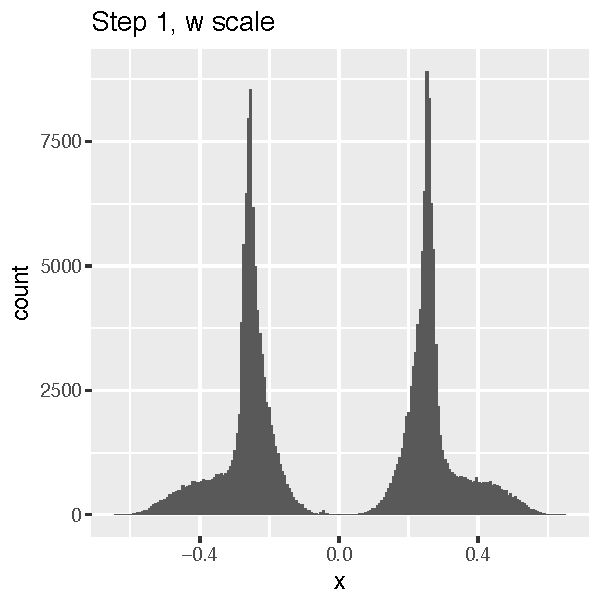
\includegraphics[width=0.16\linewidth]{Figs/trc_1}
  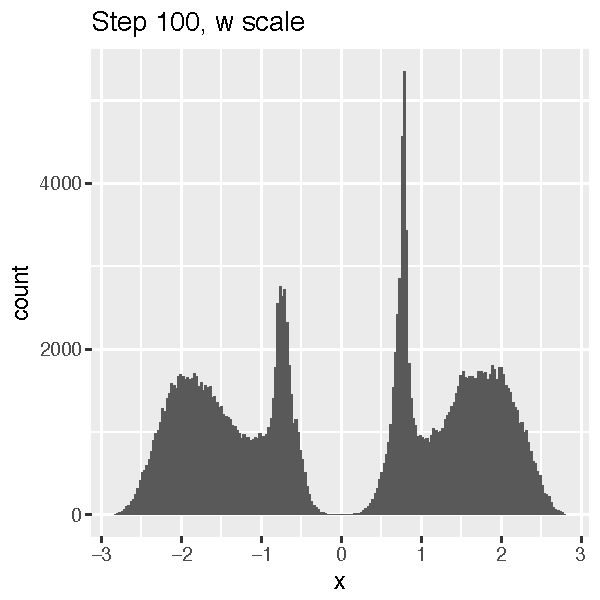
\includegraphics[width=0.16\linewidth]{Figs/trc_100}
  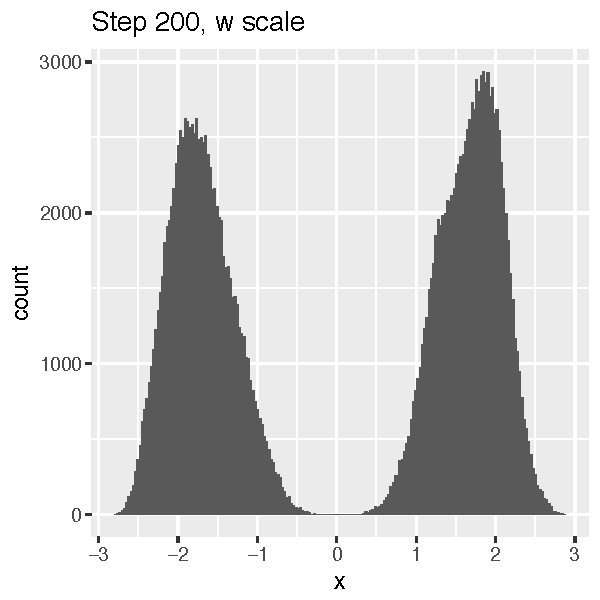
\includegraphics[width=0.16\linewidth]{Figs/trc_200}
  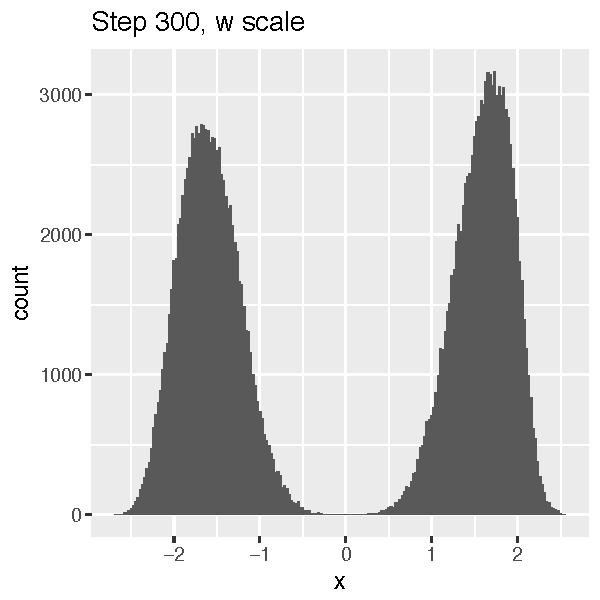
\includegraphics[width=0.16\linewidth]{Figs/trc_300}
  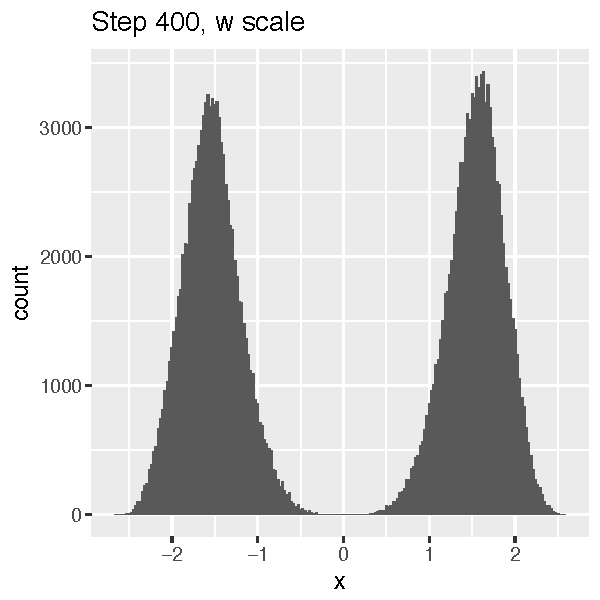
\includegraphics[width=0.16\linewidth]{Figs/trc_400}
  \caption{Same histograms as in Fig.~\ref{fig:hist_tr} after
    removing inlying anomalies.}
  \label{fig:hist_trc}
\end{figure}

